%
%===============>>  ГРУППА 10-2 МОДУЛЬ 4  <<=============
%
\setmodule{4}
%
%===============>>  Занятие 1  <<===============
%
\begin{class}[number=1]
	\begin{listofex}
		%		В ДЗ №1
		%		\item Вычислить рациональным способом:
		%		\begin{enumcols}[itemcolumns=3]
		%			\item \( \sqrt{16+4\cdot4\cdot24} \)
		%			\item \( \sqrt{83^3\cdot2^2-83^2\cdot2^3} \)
		%			\item \( \sqrt{50^2-4\cdot7\cdot7} \)
		%		\end{enumcols}
		\item Построить график функции \( y=2x-5 \).
		\begin{enumcols}[itemcolumns=1]
			\item Принадлежит ли точка с координатами \( (112;217) \) графику этой функции?
			\item Найти точку пересечения графика данной функции с графиком функции \( y=4x-1 \).
		\end{enumcols}
		\item Построить графики функций \( f(x)=x^2-2x+1 \) и \( g(x)=x^2+6x+8 \).\\
		Выберите верные утверждения:
		\begin{enumcols}[itemcolumns=4]
			\item \( f(-1)>f(1) \);
			\item \( g(-1)<f(-1) \);
			\item \( g(-2)=f(1) \);
			\item \( f(3)<g(-5) \);
		\end{enumcols}
		\begin{enumcols}[itemcolumns=1, resume]
			\item график функции \( f(x) \) возрастает на промежутке \( [0;+\infty) \);
			\item график функции \( g(x) \) убывает на промежутке \( [-9;-4] \);
			\item промежуток возрастания функции \( f(x) \) входит в промежуток возрастания функции \( g(x) \);
			\item \( f(x)=4 \) при \( x=3 \);
			\item наименьшее значение функция \( f(x) \) принимает в \( x=-1 \);
			\item наименьшее значение \( f(x) \) меньше наименьшего значения \( g(x) \);
			\item корнем уравнения \( f(x)=9 \) является только \( x=-2 \);
			\item \( f(x)\ge0 \) при любом \( x \);
			\item \( g(x)\le0 \) при \( x\in[-4;-2] \);
			\item график функции \( g(x) \) пересекается c осью \( Y \) в точке \( (0;4) \).
		\end{enumcols}
		\item Решить систему неравенств:
		\begin{enumcols}[itemcolumns=2]
			\item
			\( \left\{
			\begin{array}{l}
				3(x-1)-2(2-3x)>5x-3,\\
				8x-3(2x+5)<2(x-7).
			\end{array}
			\right. \)
			\item
			\( \left\{
			\begin{array}{l}
				12x-3(x-5)>2x+1,\\
				(x-7)(x+12)\le0.
			\end{array}
			\right. \)
		\end{enumcols}
		\item При каких значениях переменной выражение \( \sqrt{4x+1}+\sqrt{2-3x} \) имеет смысл?
		\item Построить график функции \( f(x)=\sqrt{x-4}+1 \).
		\begin{enumcols}[itemcolumns=1]
			\item определить область определения и область значений функции;
			\item сравнить \( f(7) \) и \( f(12) \);
			\item вычислить \( f(x)=26 \)
			\item существует ли \( x \), при котором \( f(x)=-1 \)? Объясните это графически и аналитически.
		\end{enumcols}
		\item Построить график функции \( y=x-|2x+1|-2 \).
		\begin{enumcols}[itemcolumns=1]
			\item найти точку минимума и наименьшее значение данной функции;
			\item определить промежутки возрастания и убывания функции;
			\item найти точки пересечения данного графика с графиком функции \( y=x-5 \).
		\end{enumcols}
		\item Баржа прошла по течению реки 48 км и, повернув обратно, прошла ещё 36 км, затратив на весь путь 6 часов. Найдите собственную скорость баржи, если скорость течения реки равна 5 км/ч.
	\end{listofex}
\end{class}
\newpage
%
%===============>>  Занятие 2  <<===============
%
\begin{class}[number=2]
	\begin{listofex}
%		В ДЗ
%		\item Постройте графики функции \( y=4x-1 \) и \( y=-\dfrac{1}{2}x+2,5 \). Графически определите точку пересечения этих графиков. Во сколько раз ордината точки пересечения больше абсциссы?
		\item Найдите точку пересечения графиков функций \( y=12x-70 \) и \( y=6x+2 \).
		\item Постройте график функции \( f(x)=x^2-6x+8 \). Выберите верные утверждения:
		\begin{enumcols}[itemcolumns=1]
			\item График функции возрастает на промежутке \( [4;+\infty) \);
			\item График функции убывает на промежутке \( [-7;7] \);
			\item \( f(-4)<f(4) \);
			\item \( f(-1)=f(3) \);
			\item \( f(x)\ge0 \) при \( x\ge4 \);
			\item \( f(x)\ge0 \) только при \( x\ge4 \);
			\item Данный график функции пересекается с графиком \( y=-x-8 \) в двух точках.
		\end{enumcols}
		\item Подставьте вместо знака \( * \) число так, чтобы функция \( y=2x^2-3x+* \) проходила через точку с координатами \( (4;15) \). Найдите координаты вершины этой параболы. Вычислите расстояние от вершины до точки \( (4;15) \).
		
%		В ДЗ
%		\item Решить систему неравенств:
%		\[ \left\{
%		\begin{array}{l}
%			6(x+2)-4(0,5-2x)>2x-6,\\
%			9x+x(2x+5)<2(x^2-7).
%		\end{array}
%		\right. \]

%		В ДЗ
%		\item \exercise{177}
%		\item \exercise{189}

		\item При каких значениях переменной выражение \( \sqrt{12x-6}+\sqrt{4-5x} \) имеет смысл?
		\item \exercise{1240}
		\item \exercise{24}
		\item \exercise{1855}
		\item Высота равностороннего треугольника равна \( 15\sqrt{3} \). Найдите его периметр.
	\end{listofex}
\end{class}
\newpage
%
%===============>>  Домашняя работа 1  <<===============
%
\begin{homework}[number=1]
	\begin{listofex}
		\item Вычислить рациональным способом:
		\begin{enumcols}[itemcolumns=3]
			\item \( \sqrt{16+4\cdot4\cdot24} \)
			\item \( \sqrt{83^3\cdot2^2-83^2\cdot2^3} \)
			\item \( \sqrt{50^2-4\cdot7\cdot7} \)
		\end{enumcols}
		\item Постройте графики функции \( y=4x-1 \) и \( y=-\dfrac{1}{2}x+2,5 \). Графически определите точку пересечения этих графиков. Во сколько раз ордината точки пересечения больше абсциссы?
		\item Решить систему неравенств:
		\[ \left\{
		\begin{array}{l}
			6(x+2)-4(0,5-2x)>2x-6,\\
			9x+x(2x+5)<2(x^2-7).
		\end{array}
		\right. \]
		\item \exercise{177}
		\item \exercise{189}
		\item Построить график функции \( f(x)=\sqrt{10-x}+5 \).
		\begin{enumcols}[itemcolumns=1]
			\item определить область определения и область значений функции;
			\item сравнить \( f(-6) \) и \( f(6) \);
			\item вычислить \( f(x)=17 \)
			\item существует ли \( x \), при котором \( f(x)=15 \)? Объясните это графически и аналитически.
		\end{enumcols}
		\item Постройте график функции \( f(x)=x^2+6x+5 \). Выберите верные утверждения:
		\begin{enumcols}[itemcolumns=1]
			\item График функции возрастает на промежутке \( [-5;+\infty) \);
			\item График функции убывает на промежутке \( [-7;-2,5] \);
			\item \( f(-5)<f(-1) \);
			\item \( f(0)=f(-6) \);
			\item \( f(x)\ge0 \) при \( x\ge1 \);
			\item \( f(x)\ge0 \) только при \( x\ge1 \);
			\item Данный график функции пересекается с графиком \( y=x-1 \) в двух точках.
		\end{enumcols}
	\end{listofex}
\end{homework}
\newpage
%
%===============>>  Занятие 3  <<===============
%
\begin{class}[number=3]
	\begin{listofex}
		\item Вычислить:
		\begin{enumcols}[itemcolumns=2]
			\item \( \dfrac{\left( 5^{3/5}\cdot7^{2/3} \right)^{15}}{39^9} \)
			\item \( 20^{-3,9}\cdot5^{2,9}:4^{-4,9} \)
			\item \( \dfrac{32^{-9}\cdot8^4}{\left( 4^{-8} \right)^2} \)
			\item \( \dfrac{\sqrt[3]{81}\cdot\sqrt[4]{81}}{\sqrt[12]{81}} \)
		\end{enumcols}
		\item \exercise{1867}
		\item 
		\begin{minipage}[t]{0.43\textwidth}
			На рисунке изображены графики функций \( f(x)=\dfrac{k}{x} \) и \( g(x)=ax+b \), которые пересекаются в точках \( A \) и \( B \). Найдите абсциссу точки \( B \).
		\end{minipage}
		\begin{minipage}[c]{0.1\textwidth}
			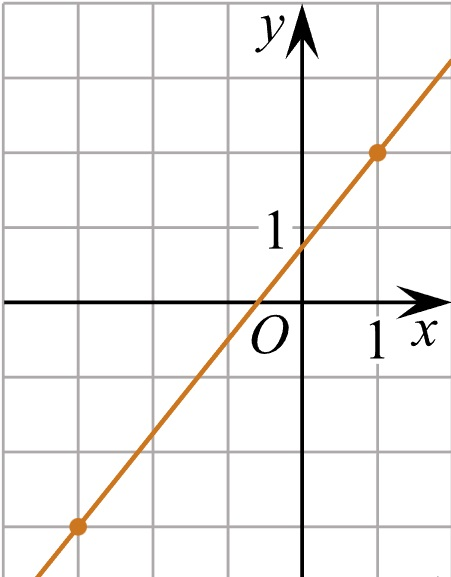
\includegraphics[align=t, width=\textwidth]{../pics/G101M4C4-1}
		\end{minipage}
		\newpage
		\item 
		\begin{minipage}[t]{0.43\textwidth}
			На рисунке изображены графики функций \( f(x)=k\sqrt{x} \). Найдите \( f(6,76) \).
		\end{minipage}
		\begin{minipage}[c]{0.1\textwidth}
			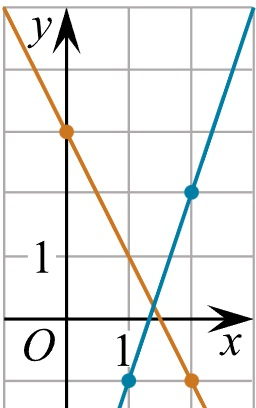
\includegraphics[align=t, width=\textwidth]{../pics/G101M4C4-2}
		\end{minipage}
		\item Решите уравнение: \( (x^2-25)\cdot\sqrt{8+2x-x^2}=(25-x^2)\cdot\sqrt{x+2} \)
		\item Расстояние между пристанями \( A \) и \( B \) равно \( 63 \) км. Из \( A \) в \( B \) по течению реки отправился плот, а через \( 1 \) час вслед за ним отправилась яхта, которая прибыла в пункт \( B \), а через \( 1 \) час отправилась обратно и возвратилась в A. К этому времени плот проплыл \( 20 \) км. Найдите скорость яхты в неподвижной воде, если скорость течения реки равна \( 2 \) км/ч. Ответ дайте в км/ч.
		\item Дан куб, сумма площадей граней которого равна \( 24 \), и дан прямоугольный
		параллелепипед \( ABCDA_1B_1C_1D_1 \). Ребро \( AB \) прямоугольного
		параллелепипеда меньше ребра куба на \( 1 \), ребро \( AD \) --- больше ребра куба
		на \( 1 \), а ребро \( AA_1 \) --- равно ребру куба. Найдите сумму площадей граней
		прямоугольного параллелепипеда \( ABCDA_1B_1C_1D_1 \).
		\item Около трапеции описана окружность. Периметр трапеции равен \( 36 \),
		средняя линия равна \( 8 \). Найдите длину боковой стороны трапеции.
	\end{listofex}
\end{class}
\newpage
%
%===============>>  Занятие 4  <<===============
% смещение на одно занятие с прошлого месяца
%\begin{class}[number=4]
%	\begin{listofex}
%		\item Пусто
%	\end{listofex}
%\end{class}
%
%===============>>  Домашняя работа 2  <<===============
%
\begin{homework}[number=2]
	\begin{listofex}
		\item 
		\begin{minipage}[t]{0.43\textwidth}
			На рисунке изображены графики двух линейных функций. Найдите абсциссу точки пересечения графиков.
		\end{minipage}
		\begin{minipage}[c]{0.1\textwidth}
			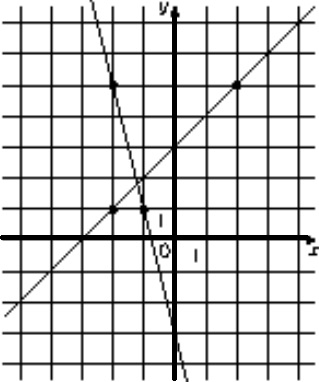
\includegraphics[align=t, width=\textwidth]{../pics/G102M4H2-1.jpg}
		\end{minipage}
		\item 
		\begin{minipage}[t]{0.43\textwidth}
			На рисунке изображены графики двух линейных функций. Найдите абсциссу точки пересечения графиков.
		\end{minipage}
		\begin{minipage}[c]{0.1\textwidth}
			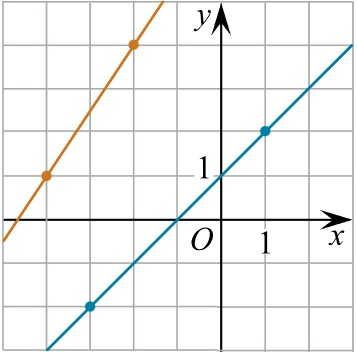
\includegraphics[align=t, width=\textwidth]{../pics/G102M4H2-2.jpg}
		\end{minipage}
		\item
		\begin{minipage}[t]{0.43\textwidth}
			На рисунке изображён график функции вида \(f(x)=a+\dfrac{b}{x-c}\), где числа \(a, b, c\) --- целые. Найдите \(f(-6)\).
		\end{minipage}
		\begin{minipage}[c]{0.1\textwidth}
			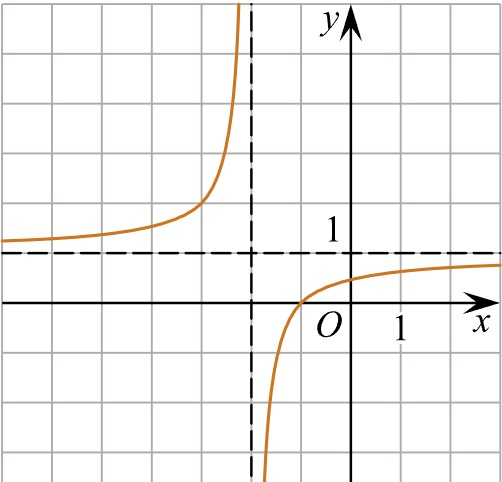
\includegraphics[align=t, width=\textwidth]{../pics/G101M4H2-10.jpg}
		\end{minipage}
		\item
		\begin{minipage}[t]{0.43\textwidth}
			На рисунке изображён график функции вида \(f(x)=\dfrac{ax+b}{x+c}\), где числа \(a, b, c\) --- целые. Найдите \(a\).
		\end{minipage}
		\begin{minipage}[c]{0.1\textwidth}
			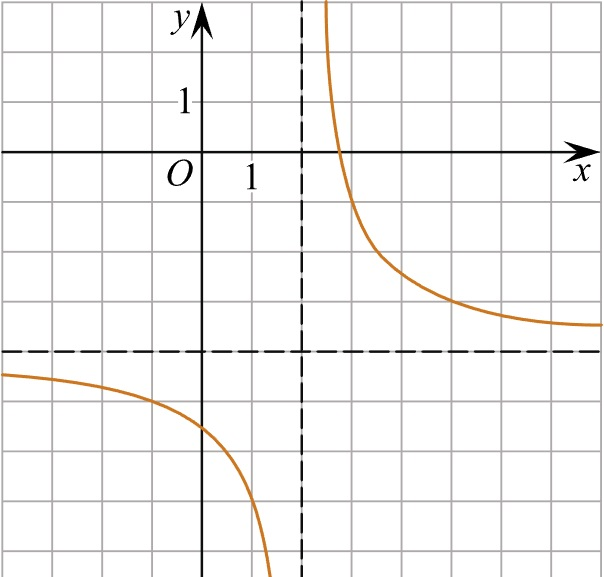
\includegraphics[align=t, width=\textwidth]{../pics/G101M4H2-11.jpg}
		\end{minipage}
		\newpage
		\item
		\begin{minipage}[t]{0.43\textwidth}
			На рисунке изображён график функции вида \(f(x)=ax+|bx+c|+d\), где числа \(a, b, c, d\) --- целые. Найдите корень уравнения \(ax+d=0\).
		\end{minipage}
		\begin{minipage}[c]{0.1\textwidth}
			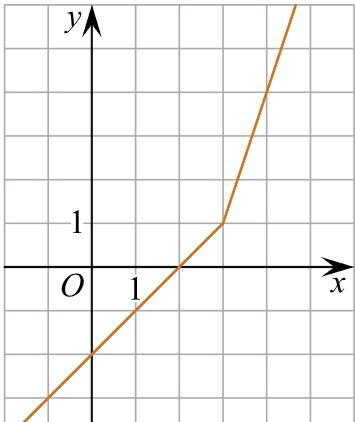
\includegraphics[align=t, width=\textwidth]{../pics/G101M4C5-8.jpg}
		\end{minipage}
		\item
		\begin{minipage}[t]{0.43\textwidth}
			На рисунке изображён график функции вида \(f(x)=ax-|bx+c|+d\), где числа \(a, b, c, d\) --- целые. Найдите корень уравнения \(ax=d\).
		\end{minipage}
		\begin{minipage}[c]{0.1\textwidth}
			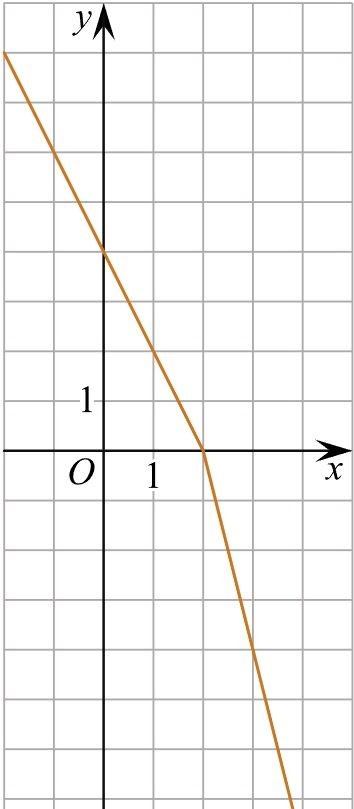
\includegraphics[align=t, width=\textwidth]{../pics/G101M4H2-7.jpg}
		\end{minipage}
		\item В ходе распада радиоактивного изотопа его масса уменьшается по закону \( m(t)=m_0\cdot2^{-t/T} \), где \( m_0 \) - начальная масса изотопа,  \( t \) - время, прошедшее от начального момента, \( T \) - период полураспада. В начальный момент времени масса изотопа \( 112 \) мг. Период его полураспада составляет \( 9  \) мин. Найдите, через сколько минут масса изотопа будет равна \( 14  \) мг.
		\item \exercise{756}
	\end{listofex}
	\newpage
\end{homework}
\newpage
%
%===============>>  Занятие 5  <<===============
%
\begin{class}[number=5]
	\begin{listofex}
		\newpage
		\item
<<<<<<< HEAD
<<<<<<< HEAD
		\begin{minipage}[t]{\bodywidth}
			На рисунке изображён график функции вида \[ f(x)=ax^2+bx+c, \] где числа \(a, b, c\) --- целые. Найдите значение \(f(6,5)\).
=======
=======
>>>>>>> b62000d7fbf6a0891bc1e1a83262b30711599274
		\begin{minipage}[t]{0.43\textwidth}
			На рисунке изображён график функции вида \(f(x)=\dfrac{k}{x}+a\). Найдите, при каком значение \(x)\) значение функции равно \(0,8\).
		\end{minipage}
		\begin{minipage}[c]{0.25\textwidth}
			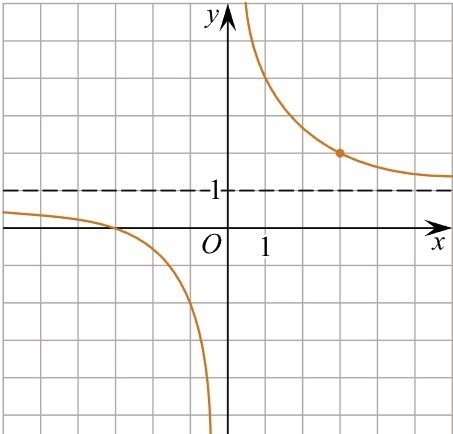
\includegraphics[align=t, width=\textwidth]{../pics/G101M4C5-1.jpg}
		\end{minipage}
		\item
		\begin{minipage}[t]{0.43\textwidth}
			На рисунке изображён график функции вида \(f(x)=\dfrac{a}{x+b}+c\), где числа \(a, b, c\) --- целые. Найдите \(f(9)\).
<<<<<<< HEAD
>>>>>>> 1b9278f8ffbcfbf3d0e771c55020f1e26dc94853
		\end{minipage}
		\hspace{0.05\linewidth}
		\begin{minipage}[t]{\picwidth}
			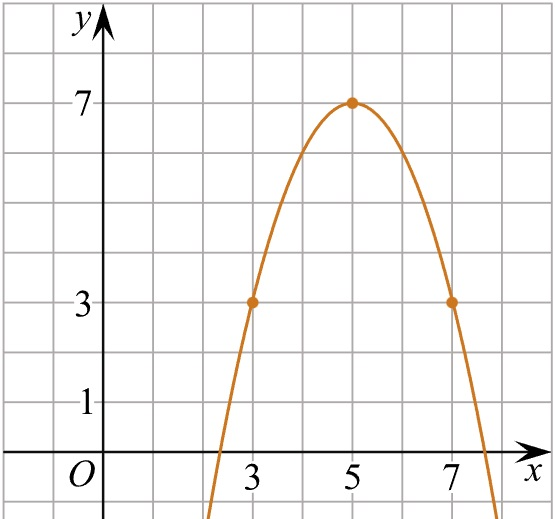
\includegraphics[align=t, width=\textwidth]{../pics/G101M4H2-5.jpg}
		\end{minipage}
		\item
<<<<<<< HEAD
		\begin{minipage}[t]{\bodywidth}
			На рисунке изображён график функции вида \[ f(x)=\dfrac{k}{x}+a. \] Найдите, при каком значение \( x \) значение функции равно \(0,8\).
=======
		\begin{minipage}[t]{0.43\textwidth}
			На рисунке изображён график функции вида \(f(x)=\dfrac{a}{x+b}+c\), где числа \(a, b, c\) --- целые. Найдите \(f(4)\).
>>>>>>> 1b9278f8ffbcfbf3d0e771c55020f1e26dc94853
		\end{minipage}
		\hspace{0.05\linewidth}
		\begin{minipage}[t]{\picwidth}
			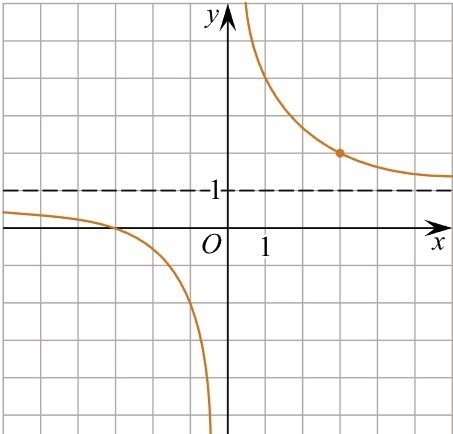
\includegraphics[align=t, width=\linewidth]{../pics/G101M4C5-1.jpg}
		\end{minipage}
		\item
<<<<<<< HEAD
		\begin{minipage}[t]{\bodywidth}
			На рисунке изображён график функции вида \[ f(x)=\dfrac{k}{x+b}+a, \] где числа \(a, b, c\) --- целые. Найдите \(f(9)\).
=======
		\begin{minipage}[t]{0.43\textwidth}
			На рисунке изображён график функции вида \(f(x)=\dfrac{ax+b}{x+c}\), где числа \(a, b, c\) --- целые. Найдите \(a\).
>>>>>>> 1b9278f8ffbcfbf3d0e771c55020f1e26dc94853
		\end{minipage}
		\hspace{0.05\linewidth}
		\begin{minipage}[t]{\picwidth}
			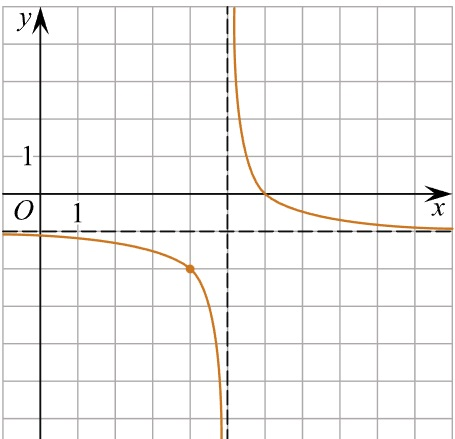
\includegraphics[align=t, width=\linewidth]{../pics/G101M4C5-2.jpg}
		\end{minipage}
		\item
<<<<<<< HEAD
		\begin{minipage}[t]{\bodywidth}
			На рисунке изображён график функции вида \[ f(x)=\dfrac{k}{x+b}+a, \] где числа \(a, b, c\) --- целые. Найдите \(f(4)\).
=======
		\begin{minipage}[t]{0.43\textwidth}
			На рисунке изображён график функции вида \(f(x)=\dfrac{ax+b}{x+c}\), где числа \(a, b, c\) --- целые. Найдите \(a\).
>>>>>>> 1b9278f8ffbcfbf3d0e771c55020f1e26dc94853
=======
		\begin{minipage}[t]{\bodywidth}
			На рисунке изображён график функции вида \[ f(x)=ax^2+bx+c, \] где числа \(a, b, c\) --- целые. Найдите значение \(f(6,5)\).
		\begin{minipage}[t]{0.43\textwidth}
			На рисунке изображён график функции вида \(f(x)=\dfrac{a}{x+b}+c\), где числа \(a, b, c\) --- целые. Найдите \(f(4)\).
		\begin{minipage}[t]{\bodywidth}
			На рисунке изображён график функции вида \[ f(x)=\dfrac{k}{x}+a. \] Найдите, при каком значение \( x \) значение функции равно \(0,8\).
		\item
		\begin{minipage}[t]{0.43\textwidth}
			На рисунке изображён график функции вида \(f(x)=\dfrac{ax+b}{x+c}\), где числа \(a, b, c\) --- целые. Найдите \(a\).
		\begin{minipage}[t]{\bodywidth}
			На рисунке изображён график функции вида \[ f(x)=\dfrac{k}{x+b}+a, \] где числа \(a, b, c\) --- целые. Найдите \(f(9)\).
		\begin{minipage}[t]{0.43\textwidth}
			На рисунке изображён график функции вида \(f(x)=\dfrac{ax+b}{x+c}\), где числа \(a, b, c\) --- целые. Найдите \(a\).
		\begin{minipage}[t]{\bodywidth}
			На рисунке изображён график функции вида \[ f(x)=\dfrac{k}{x+b}+a, \] где числа \(a, b, c\) --- целые. Найдите \(f(4)\).
>>>>>>> b62000d7fbf6a0891bc1e1a83262b30711599274
		\end{minipage}
		\hspace{0.05\linewidth}
		\begin{minipage}[t]{\picwidth}
			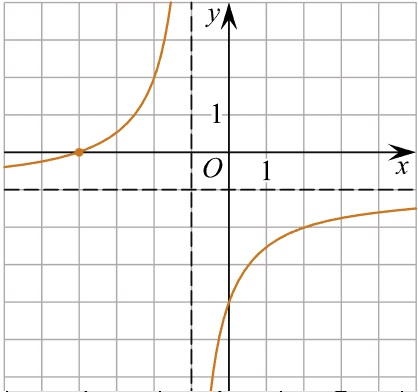
\includegraphics[align=t, width=\linewidth]{../pics/G101M4C5-3.jpg}
		\end{minipage}
		\item
<<<<<<< HEAD
<<<<<<< HEAD
		\begin{minipage}[t]{\bodywidth}
			На рисунке изображён график функции вида \[ f(x)=\dfrac{ax+b}{x+c}, \] где числа \(a, b, c\) --- целые. Найдите \(a\).
=======
		\begin{minipage}[t]{0.43\textwidth}
			На рисунке изображён график функции вида \(f(x)=ax+|bx+c|+d\), где числа \(a, b, c, d\) --- целые. Найдите корень уравнения \(ax+d=0\).
>>>>>>> 1b9278f8ffbcfbf3d0e771c55020f1e26dc94853
		\end{minipage}
		\hspace{0.05\linewidth}
		\begin{minipage}[t]{\picwidth}
			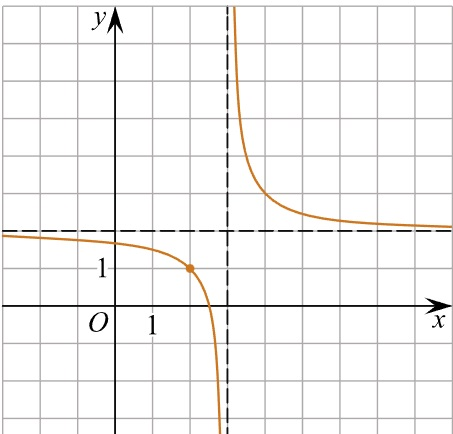
\includegraphics[align=t, width=\linewidth]{../pics/G101M4C5-4.jpg}
		\end{minipage}
		\item
<<<<<<< HEAD
		\begin{minipage}[t]{\bodywidth}
			На рисунке изображён график функции вида \[ f(x)=\dfrac{ax+b}{x+c}, \] где числа \(a, b, c\) --- целые. Найдите \(a\).
=======
		\begin{minipage}[t]{0.43\textwidth}
			На рисунке изображён график функции вида \(f(x)=ax+|bx+c|+d\), где числа \(a, b, c, d\) --- целые. Найдите корень уравнения \(ax+d=0\).
>>>>>>> 1b9278f8ffbcfbf3d0e771c55020f1e26dc94853
		\end{minipage}
		\hspace{0.05\linewidth}
		\begin{minipage}[t]{\picwidth}
			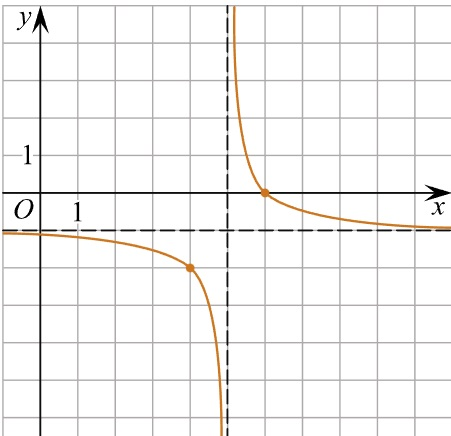
\includegraphics[align=t, width=\linewidth]{../pics/G101M4C5-5.jpg}
		\end{minipage}
		\item
<<<<<<< HEAD
		\begin{minipage}[t]{\bodywidth}
			На рисунке изображён график функции вида \[ f(x)=ax+|bx+c|+d, \] где числа \(a, b, c, d\) --- целые.\\ Найдите корень уравнения \(ax+d=0\).
=======
		\begin{minipage}[t]{0.43\textwidth}
			На рисунке изображён график функции вида \(f(x)=ax+|bx+c|+d\), где числа \(a, b, c, d\) --- целые. Найдите корень уравнения \(ax+d=0\).
>>>>>>> 1b9278f8ffbcfbf3d0e771c55020f1e26dc94853
=======
		\begin{minipage}[t]{0.43\textwidth}
			На рисунке изображён график функции вида \(f(x)=ax+|bx+c|+d\), где числа \(a, b, c, d\) --- целые. Найдите корень уравнения \(ax+d=0\).
		\begin{minipage}[t]{\bodywidth}
			На рисунке изображён график функции вида \[ f(x)=\dfrac{ax+b}{x+c}, \] где числа \(a, b, c\) --- целые. Найдите \(a\).
		\begin{minipage}[t]{0.43\textwidth}
			На рисунке изображён график функции вида \(f(x)=ax+|bx+c|+d\), где числа \(a, b, c, d\) --- целые. Найдите корень уравнения \(ax+d=0\).
		\begin{minipage}[t]{\bodywidth}
			На рисунке изображён график функции вида \[ f(x)=\dfrac{ax+b}{x+c}, \] где числа \(a, b, c\) --- целые. Найдите \(a\).
		\item
		\begin{minipage}[t]{0.43\textwidth}
			На рисунке изображён график функции вида \(f(x)=ax+|bx+c|+d\), где числа \(a, b, c, d\) --- целые. Найдите корень уравнения \(ax+d=0\).
		\begin{minipage}[t]{\bodywidth}
			На рисунке изображён график функции вида \[ f(x)=ax+|bx+c|+d, \] где числа \(a, b, c, d\) --- целые.\\ Найдите корень уравнения \(ax+d=0\).
>>>>>>> b62000d7fbf6a0891bc1e1a83262b30711599274
		\end{minipage}
		\hspace{0.05\linewidth}
		\begin{minipage}[t]{\picwidth}
			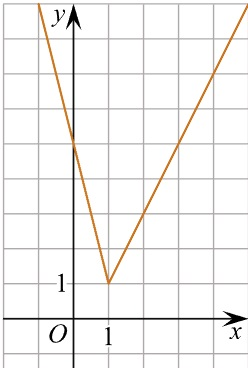
\includegraphics[align=t, width=\linewidth]{../pics/G101M4C5-6.jpg}
		\end{minipage}
		\item
<<<<<<< HEAD
<<<<<<< HEAD
		\begin{minipage}[t]{\bodywidth}
			На рисунке изображён график функции вида \[ f(x)=ax+|bx+c|+d, \] где числа \(a, b, c, d\) --- целые.\\ Найдите корень уравнения \(ax+d=8\).
		\end{minipage}
		\hspace{0.05\linewidth}
		\begin{minipage}[t]{\picwidth}
			\includegraphics[align=t, width=\linewidth]{../pics/G101M4C5-7.jpg}
=======
=======
>>>>>>> b62000d7fbf6a0891bc1e1a83262b30711599274
		\begin{minipage}[t]{0.43\textwidth}
			На рисунке изображён график функции вида \(f(x)=ax+|bx+c|+d\), где числа \(a, b, c, d\) --- целые. Найдите корень уравнения \(ax+d=19\).
		\end{minipage}
		\begin{minipage}[c]{0.17\textwidth}
			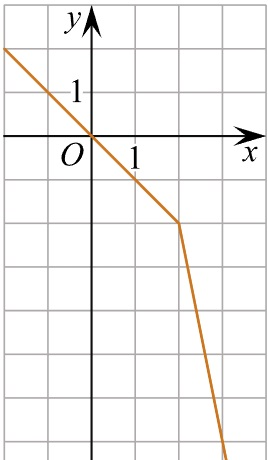
\includegraphics[align=t, width=\textwidth]{../pics/G101M4C5-9.jpg}
		\end{minipage}
		\newpage
		\item
		\begin{minipage}[t]{0.43\textwidth}
			На рисунке изображён график функции вида \(f(x)=ax+|bx+c|+d\), где числа \(a, b, c, d\) --- целые. Найдите корень уравнения \(ax=d\).
		\end{minipage}
		\begin{minipage}[c]{0.27\textwidth}
			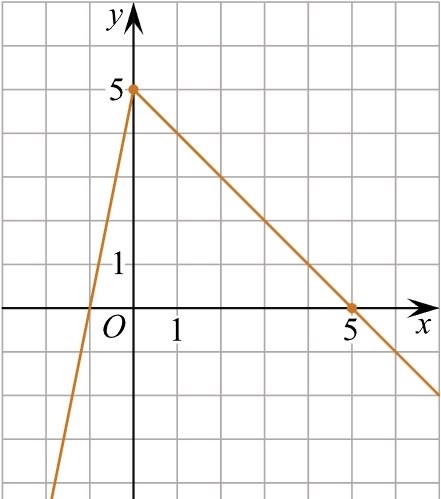
\includegraphics[align=t, width=\textwidth]{../pics/G101M4C5-10.jpg}
<<<<<<< HEAD
>>>>>>> 1b9278f8ffbcfbf3d0e771c55020f1e26dc94853
=======
		\begin{minipage}[t]{\bodywidth}
			На рисунке изображён график функции вида \[ f(x)=ax+|bx+c|+d, \] где числа \(a, b, c, d\) --- целые.\\ Найдите корень уравнения \(ax+d=8\).
		\end{minipage}
		\hspace{0.05\linewidth}
		\begin{minipage}[t]{\picwidth}
			\includegraphics[align=t, width=\linewidth]{../pics/G101M4C5-7.jpg}
>>>>>>> b62000d7fbf6a0891bc1e1a83262b30711599274
		\end{minipage}
		\item Высота над землeй подброшенного вверх мяча меняется по закону \(h(t)=1,6+8t-5t^2\) где \(h\) --- высота в метрах, \(t\) --- время в секундах, прошедшее с момента броска. Сколько секунд мяч будет
		находиться на высоте не менее трeх метров?
	\end{listofex}
\end{class}
\newpage
%
%===============>>  Домашняя работа 3  <<===============
%
%\begin{homework}[number=3]
%	\begin{listofex}
%		\item 
%	\end{listofex}
%\end{homework}
%\newpage
%\title{Подготовка к проверочной работе}
%\begin{listofex}
%	
%\end{listofex}
%
%===============>>  Занятие 6  <<===============
%
\begin{class}[number=6]
	\begin{listofex}
		\item Решить систему неравенств:
		\[ \left\{
		\begin{array}{l}
			5(4x+3)-3(4x+5)\le8x+9,\\
			\dfrac{x+2}{4}+\dfrac{x+4}{2}\ge\dfrac{x+3}{5}+\dfrac{x+5}{3}.
		\end{array}
		\right. \]
		\item Решите двойное неравенство: \( 2x+3\le5x^2-9x+5\le7x+2 \).
		\item Гоночный автомобиль разгоняется на прямолинейном участке шоссе с постоянным ускорением \( a \) км/ч\( ^2 \). Скорость \( v \)  в конце пути вычисляется по формуле \( v=\sqrt{2la} \), где \( l \) – пройденный автомобилем путь в км. Определите ускорение, с которым должен двигаться автомобиль, чтобы, проехав \( 250 \) метров, приобрести скорость \( 60 \)км/ч. Ответ выразите в км/ч\( ^2 \).
		\item
		\begin{minipage}[t]{\bodywidth}
			На рисунке изображён график функции \(f(x)=kx+b\). Найдите \(f(-9)\).
		\end{minipage}
		\hspace{0.02\linewidth}
		\begin{minipage}[t]{\picwidth}
			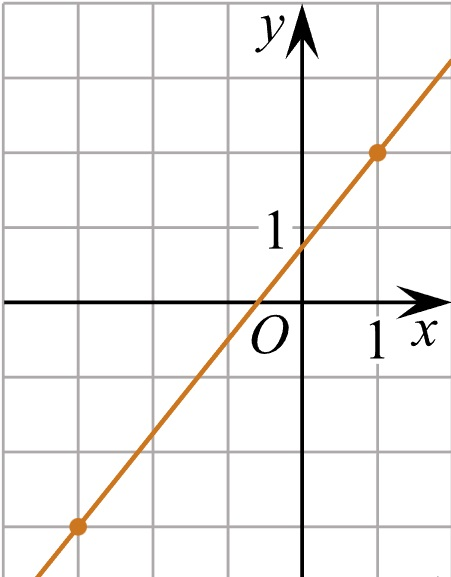
\includegraphics[align=t, width=\textwidth]{../pics/G101M4C4-1.jpg}
		\end{minipage}
		\item
		\begin{minipage}[t]{\bodywidth}
			На рисунке изображён график функции вида \(f(x)=ax^2+bx+c\), где числа \(a, b, c\) --- целые. Найдите значение \(f\left( -\mfrac{1}{1}{2} \right)\).
		\end{minipage}
		\hspace{0.02\linewidth}
		\begin{minipage}[t]{\picwidth}
			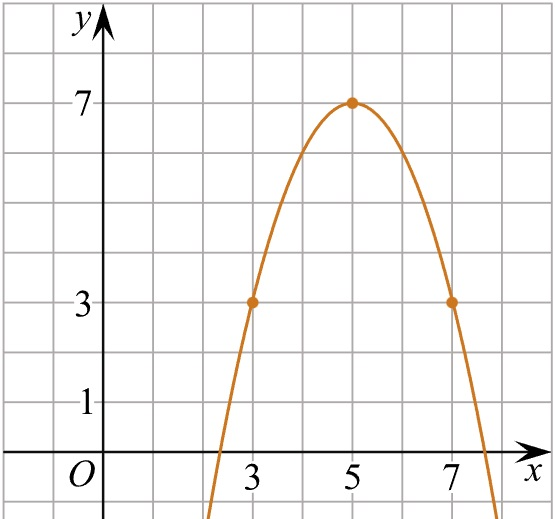
\includegraphics[align=t, width=\linewidth]{../pics/G101M4H2-5.jpg}
		\end{minipage}
		\item
		\begin{minipage}[t]{\bodywidth}
			На рисунке изображён график функции вида \[ f(x)=ax+|bx+c|+d, \] где числа \(a, b, c, d\) --- целые. Найдите корень уравнения \(ax+d=-15\).
		\end{minipage}
		\hspace{0.02\linewidth}
		\begin{minipage}[t]{\picwidth}
			\includegraphics[align=t, width=\linewidth]{pics/G101M4C5-7.jpg}
		\end{minipage}
		\item
		\begin{minipage}[t]{\bodywidth}
			На рисунке изображён график функции вида \[ f(x)=ax+|bx+c|+d, \] где числа \(a, b, c, d\) --- целые. Найдите корень уравнения \(bx+c=2\).
		\end{minipage}
		\hspace{0.02\linewidth}
		\begin{minipage}[t]{\picwidth}
			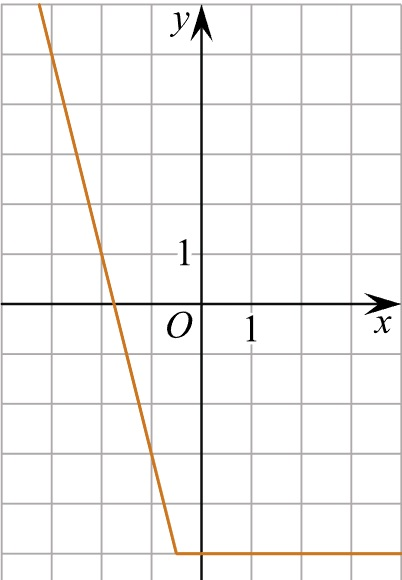
\includegraphics[align=t, width=\linewidth]{../pics/G101M4H2-6.jpg}
		\end{minipage}
		\item
		\begin{minipage}[t]{\bodywidth}
			На рисунке изображён график функции вида \[ f(x)=ax-|bx+c|+d, \] где числа \(a, b, c, d\) --- целые. Найдите корень уравнения \(ax+d=-2\).
		\end{minipage}
		\hspace{0.02\linewidth}
		\begin{minipage}[t]{\picwidth}
			\includegraphics[align=t, width=\linewidth]{pics/G101M4C6-8.jpg}
		\end{minipage}
		\item
		\begin{minipage}[t]{\bodywidth}
			На рисунке изображён график функции вида \[ f(x)=\dfrac{a}{x+b}+c, \] где числа \(a, b, c\) --- целые. Найдите значение \(x\), при котором \(f(x)=-5\).
		\end{minipage}
		\hspace{0.02\linewidth}
		\begin{minipage}[t]{\picwidth}
			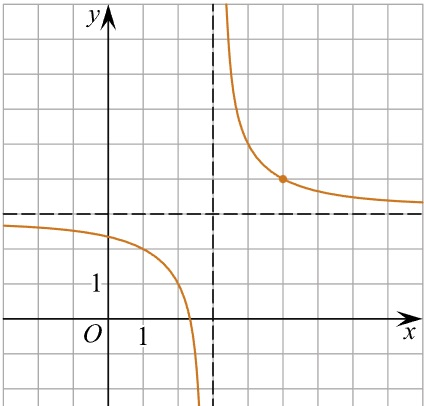
\includegraphics[align=t, width=\linewidth]{../pics/G101M4C6-2.jpg}
		\end{minipage}
		\begin{minipage}[t]{0.43\textwidth}
			На рисунке изображён график функции вида \(f(x)=ax+|bx+c|+d\), где числа \(a, b, c, d\) --- целые. Найдите корень уравнения \(ax+d=10\).
		\end{minipage}
		\begin{minipage}[c]{0.1\textwidth}
			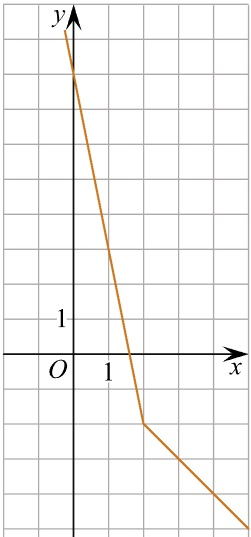
\includegraphics[align=t, width=\textwidth]{../pics/G101M4C6-1.jpg}
		\end{minipage}
		\item
		\begin{minipage}[t]{0.43\textwidth}
			На рисунке изображён график функции вида \(f(x)=ax+|bx+c|+d\), где числа \(a, b, c, d\) --- целые. Найдите корень уравнения \(ax+d=-15\).
		\end{minipage}
		\begin{minipage}[c]{0.1\textwidth}
			\includegraphics[align=t, width=\textwidth]{../pics/G101M4C5-7.jpg}
		\end{minipage}
		\item
		\begin{minipage}[t]{0.43\textwidth}
			На рисунке изображён график функции вида \(f(x)=ax+|bx+c|+d\), где числа \(a, b, c, d\) --- целые. Найдите корень уравнения \(bx+c=2\).
		\end{minipage}
		\begin{minipage}[c]{0.1\textwidth}
			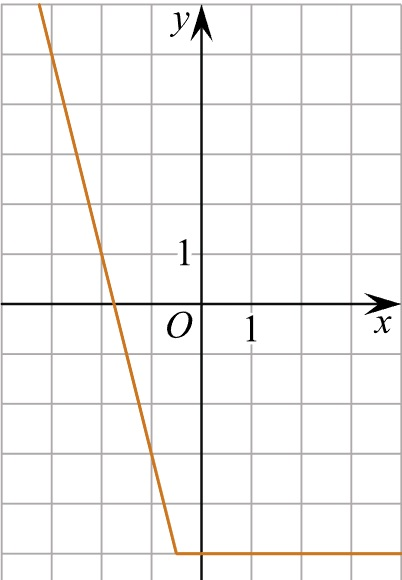
\includegraphics[align=t, width=\textwidth]{../pics/G101M4H2-6.jpg}
		\end{minipage}
		\item
		\begin{minipage}[t]{0.43\textwidth}
			На рисунке изображён график функции вида \(f(x)=ax-|bx+c|+d\), где числа \(a, b, c, d\) --- целые. Найдите корень уравнения \(ax+d=-2\).
		\end{minipage}
		\begin{minipage}[c]{0.1\textwidth}
			\includegraphics[align=t, width=\textwidth]{../pics/G101M4C6-8.jpg}
		\end{minipage}
		\item
		\begin{minipage}[t]{0.43\textwidth}
			На рисунке изображён график функции вида \(f(x)=\dfrac{a}{x+b}+c\), где числа \(a, b, c\) --- целые. Найдите значение \(x\), при котором \(f(x)=2,5\).
		\end{minipage}
		\begin{minipage}[c]{0.1\textwidth}
			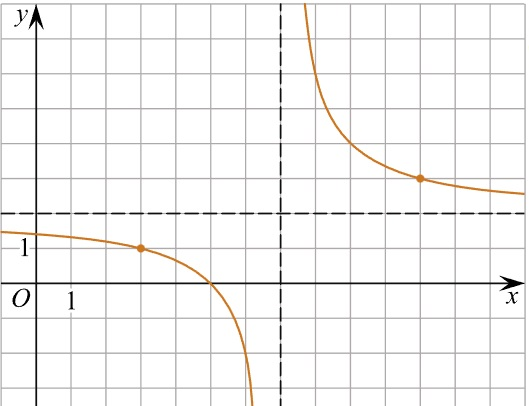
\includegraphics[align=t, width=\textwidth]{../pics/G101M4C6-3.jpg}
		\end{minipage}
		\item
		\begin{minipage}[t]{0.43\textwidth}
			На рисунке изображён график функции вида \(f(x)=\dfrac{a}{x+b}+c\), где числа \(a, b, c\) --- целые. Найдите значение \(x\), при котором \(f(x)=-1,125\).
		\end{minipage}
		\begin{minipage}[c]{0.1\textwidth}
			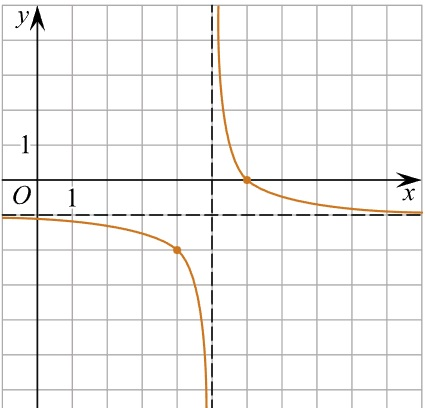
\includegraphics[align=t, width=\textwidth]{../pics/G101M4C6-4.jpg}
		\end{minipage}
		\item
		\begin{minipage}[t]{\bodywidth}
			На рисунке изображён график функции вида \[ f(x)=\dfrac{ax+b}{x+c}, \] где числа \(a, b, c\) --- целые. Найдите \(b\).
		\end{minipage}
		\hspace{0.02\linewidth}
		\begin{minipage}[t]{\picwidth}
			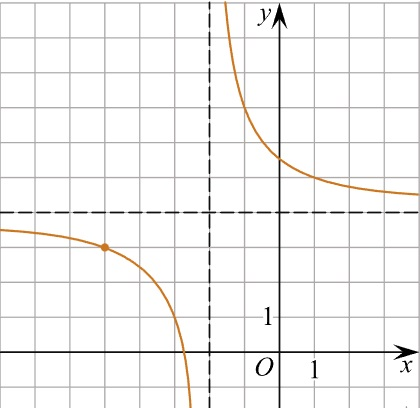
\includegraphics[align=t, width=\linewidth]{../pics/G101M4C6-5.jpg}
		\end{minipage}
%		\item Некоторая компания продает свою продукцию по цене\(  p=500  \)руб. за единицу, переменные затраты на производство одной единицы продукции составляют  \( v=300 \) руб., постоянные расходы предприятия \( f=700000 \) руб. в месяц. Месячная операционная прибыль предприятия (в рублях) вычисляется по формуле  \( \pi(q)=q(p-v)-f \). Определите месячный объeм производства\(  q \) (единиц продукции), при котором месячная операционная прибыль предприятия будет равна \( 300000 \) руб.
%		\item Зависимость объёма спроса \( q \) (единиц в месяц) на продукцию предприятия – монополиста от цены \( p \) (тыс. руб.) задаётся формулой \( q=100-10p \). Выручка предприятия за месяц \( r \) (в тыс. руб.) вычисляется по формуле \( r(p)=q\cdot p \). Определите наибольшую цену \( p \), при которой месячная выручка \( r(p) \) составит не менее \( 240 \) тыс. руб. Ответ приведите в тыс. руб.
%		\item По закону Ома для полной цепи сила тока, измеряемая в амперах, равна \( I=\dfrac{\sigma}{R+r} \), где \(\sigma\) – ЭДС источника (в вольтах), \(r=2\) Ом – его внутреннее сопротивление, \(R\) – сопротивление цепи (в омах). При каком наименьшем сопротивлении цепи сила тока будет составлять не более \(40\% \) от силы тока короткого замыкания \( I_{кз} =\dfrac{\sigma}{r}\)? (Ответ выразите в омах).
%		\item Расстояние (в км) от наблюдателя, находящегося на небольшой высоте \( h \) километров над землeй, до наблюдаемой им линии горизонта вычисляется по формуле \( l=\sqrt{2Rh} \), где \( R = 6400 \) (км) – радиус Земли. С какой высоты горизонт виден на расстоянии \(4\) километра? Ответ выразите в километрах.
%		\item В ходе распада радиоактивного изотопа его масса уменьшается по закону \( m(t)=m_0\cdot2^{-t/T} \), где \( m_0 \) - начальная масса изотопа,  \( t \) - время, прошедшее от начального момента, \( T \) - период полураспада. В начальный момент времени масса изотопа \( 52 \) мг. Период его полураспада составляет \( 9  \) мин. Найдите, через сколько минут масса изотопа будет равна \( 13  \) мг.
%		\item Расстояние от наблюдателя, находящегося на небольшой высоте  h километров над землёй, до наблюдаемой им линии горизонта вычисляется по формуле \( l=\sqrt{2Rh} \), где \( R=6400 \) км - радиус Земли. С какой высоты горизонт виден на расстоянии \( 32 \) километра? Ответ выразите в километрах.
	\end{listofex}
\end{class}
\newpage
%
%===============>>  Проверочная работа  <<===============
%
%\begin{exam}
%	\begin{listofex}
%		\item \exercise{1251}
%		\item Расстояние от наблюдателя, находящегося на небольшой высоте  h километров над землёй, до наблюдаемой им линии горизонта вычисляется по формуле \( l=\sqrt{2Rh} \), где \( R=6400 \) км - радиус Земли. С какой высоты горизонт виден на расстоянии \( 64 \) километра? Ответ выразите в километрах.
%		\newpage
%		\item Автомобиль разгоняется на прямолинейном участке шоссе с постоянным ускорением \( a \) км/ч\( ^2 \) . Скорость вычисляется по формуле \( v=\sqrt{2la} \), где \( l \) -- пройденный автомобилем путь. Найдите ускорение, с которым должен двигаться автомобиль, чтобы, проехав \( 0,7 \) километра, приобрести скорость \( 105 \) км/ч. Ответ выразите в км/ч\( ^2 \).
%		\item \exercise{1232}
%		\item \exercise{1244}
%	\end{listofex}
%\end{exam}